% This is LLNCS.DEM the demonstration file of
% the LaTeX macro package from Springer-Verlag
% for Lecture Notes in Computer Science,
% version 2.4 for LaTeX2e as of 16. April 2010
%
\documentclass{llncs}
%
\usepackage{makeidx}  % allows for indexgeneration
%\usepackage[T2A]{fontenc} 
%\usepackage[utf8]{inputenc}
%\usepackage[english,russian]{babel}
\usepackage{graphicx}
\usepackage{indentfirst}
\usepackage{hyperref}

%
\begin{document}

\sloppy
%
%\frontmatter          % for the preliminaries
%
%\pagestyle{headings}  % switches on printing of running heads
%\addtocmark{Hamiltonian Mechanics} % additional mark in the TOC
%
%
%\tableofcontents
%
%\mainmatter              % start of the contributions
%
\title{From Abstract Parsing to Abstract Translation}
%
%\titlerunning{Hamiltonian Mechanics}  % abbreviated title (for running head)
%                                     also used for the TOC unless
%                                     \toctitle is used
%
\author{Semyon Grigorev\inst{1} 
\and Iakov Kirilenko\inst{2}
}
%
%\authorrunning{Ivar Ekeland et al.} % abbreviated author list (for running head)
%
%%%% list of authors for the TOC (use if author list has to be modified)
\tocauthor{Semyon Grigorev
, Iakov Kirilenko
}


\institute{St. Petersburg State University \\
198504, Universitetsky prospekt 28, Peterhof, St. Petersburg, Russia. \\
\email{rsdpisuy@gmail.com}
\and
St. Petersburg State University \\
198504, Universitetsky prospekt 28, Peterhof, St. Petersburg, Russia. \\
\email{jake@math.spbu.ru}
}

\maketitle              % typeset the title of the contribution

\begin{abstract}

String-embedded language translation is one of the problems which can be faced during 
database application and information system migration. There are two approaches to 
solve this problem: static translation or translation at run time. Our research deals 
with the first one since solution for embedded language static translation problem do 
not still exists. There is an abstract parsing algorithm~\cite{AbstrParsing} for parsing of 
string-embedded language. Parsing is close problem and in this article we propose abstract 
parsing algorithm modification for application to string-embedded language translation. 
We describe modifications of the basic algorithm which allow to translate embedded languages. 
An algorithm of parsing forest minimization is also presented. We discuss some issues of 
real-world dynamic SQL queries static translation and provide possible solutions. Finally, 
we present results of implemented algorithm evaluation.

\keywords{Embedded languages, two-staged languages, string-embedded languages, abstract 
parsing,  abstract translation, LALR, dynamic SQL}
\end{abstract}

\chapter*{Введение}                         % Заголовок
\addcontentsline{toc}{chapter}{Введение}    % Добавляем его в оглавление
\textbf{Актуальность работы}

Статический анализ исходного кода является известной техникой  получения знаний о программе без её исполнения ~\cite{StaticCodeAnalysis3,StaticCodeAnalysis2,StaticCodeAnalysis1}. Статический анализ является неотъемлемой частью многих процессов, связанных с разработкой программного обеспечения (ПО), и может использоваться, например, для упрощения работы с кодом с помощью подсветки синтаксиса языка в программах, навигации по коду, реализации контекстных подсказок. Более того, статический анализ используется для обнаружения ошибок на ранних стадиях разработки, до запуска программы, а также для поиска различных семантических ошибок, которые не могут быть определены обычным синтаксическим анализом.  Также, статический анализ используется при решении задач трансформации исходного кода и реинжиниринге~\cite{reengANT}. Однако во многих языках программирования имеются конструкции, которые существенно затрудняют статический анализ. 

Например, широко используются динамические встроенные языки --- приложение, созданное на одном языке, генерирует программу на другом языке и передаёт её на выполнение в соответствующее окружение. Примерами могут служить динамические SQL-запросы к базам данных из приложений на Java, С++, С\#, формирование HTML-страниц в PHP-приложениях~\cite{DSQLISO,JSP,PHPmySQL}. Генерируемый код собирается из строк таким образом, чтобы в момент выполнения результирующая строка представляла собой корректную программу. Примеры использования встроенных языков представлены в листингах~\ref{lst:dsql1},~\ref{lst:JsJava} и~\ref{lst:PhPSqlHtml}. Следует отметить, что одна программа может генерировать код на нескольких языках (см. листинг~\ref{lst:PhPSqlHtml}). При этом возможно получение частей кода из разных источников (например, учитывать текстовый ввод пользователя, что часто используется для задания фильтров при конструировании SQL-запросов). Использование динамически формируемых программ  позволяет избежать дополнительных накладных расходов, присущих таким технологиям, как ORM\footnote{ORM или Object-Relational Mapping --- технология программирования, которая связывает базы данных с концепциями объектно-ориентированных языков программирования~\cite{ORM}.}, и достичь высокой производительности. Благодаря этому использование динамически генерируемых программ получило широкое распространение и применяется до сих пор. Вместе с этим, несмотря на появление новых технологий, динамическая генерация SQL-запросов активно используется и в настоящее время~\cite{DSQLInActiveUse}.

\fvset{frame=lines,framesep=5pt,fontsize=\small}\

\begin{listing}
    \begin{pyglist}[language=sql,numbers=left,numbersep=5pt]

CREATE PROCEDURE [dbo].[MyProc]  @TABLERes   VarChar(30)
AS
    EXECUTE ('INSERT INTO ' + @TABLERes + ' (sText1)' +
             ' SELECT ''Additional condition: '' + sName' +
             ' from #tt where sAction = ''1000000''')
GO
    \end{pyglist}
\caption{Код с использованием динамического SQL}
\label{lst:dsql1}
\end{listing} 
 
\fvset{frame=lines,framesep=5pt}
\begin{listing}
    \begin{pyglist}[language=java,numbers=left,numbersep=5pt]
import javax.script.*;  
public class InvokeScriptFunction {  
    public static void main(String[] args) throws Exception {  
        ScriptEngineManager manager = new ScriptEngineManager();  
        ScriptEngine engine = manager.getEngineByName("JavaScript");  
        // JavaScript code in a String  
        String script = 
            "function hello(name) { print('Hello, ' + name); }";  
        // evaluate script  
        engine.eval(script);  
        // javax.script.Invocable is an optional interface.  
        // Check whether your script engine implements or not!  
        // Note that the JavaScript engine implements
        // Invocable interface.  
        Invocable inv = (Invocable) engine;  
        // invoke the global function named "hello"  
        inv.invokeFunction("hello", "Scripting!!" );  
    }  
}
    \end{pyglist}
\caption{Вызов JavaScript из Java}
\label{lst:JsJava}
\end{listing}


\fvset{frame=lines,framesep=5pt}
\begin{listing}
    \begin{pyglist}[language=php,numbers=left,numbersep=5pt]

<?php
    // Embedded SQL
    $query = 'SELECT * FROM ' . $my_table; 
    $result = mysql_query($query);
    
    // HTML markup generation
    echo "<table>\n";
    while ($line = mysql_fetch_array($result, MYSQL_ASSOC)) {
        echo "\t<tr>\n";    
        foreach ($line as $col_value) {
            echo "\t\t<td>$col_value</td>\n";
        }
        echo "\t</tr>\n";
    }
    echo "</table>\n";
?>
    \end{pyglist}
\caption{Использование нескольких встроенных в PHP языков (MySQL, HTML)}
\label{lst:PhPSqlHtml}
\end{listing}



Динамически формируемые выражения часто конструируются с помощью таких операций, как конкатенация в циклах или условных предложениях, или в рекурсивных процедурах. Это затрудняет статический анализ и приводит к получению множества возможных значений для каждого выражения в момент выполнения. Вследствие этого фрагменты динамически формируемого кода воспринимаются компилятором исходного языка как простые строки, не подлежащие дополнительному анализу, а это, в свою очередь, приводит к высокой вероятности возникновения ошибок во время выполнения программы. В худшем случае такая ошибка не приведёт к прекращению работы приложения, что указало бы на проблемы, однако целостность данных при этом может оказаться нарушена. Более того, использование динамически формируемых выражений затрудняет не только разработку информационных систем, так и также и реинжиниринг, поскольку в последнем случае важно автоматизировать перенос системы на новые зыки и платформы, что невозможно без качественного статического анализа. Например, при наличии в коде приложения динамически формируемых SQL-запросов нельзя точно ответить на вопрос о том, с какими элементами базы данных не взаимодействует система, и удалить их. При переносе такой системы на другую СУБД необходимо гарантировать, что для всех динамически формируемых выражений значение в момент выполнения будет корректным кодом на языке новой СУБД~\cite{JSquash}. Следует отметить, что отсутствие статического анализа динамически формируемых программ не позволяет реализовывать для них стандартную функциональность интегрированных сред разработки (Integrated Development Environment, IDE) --- подсветку синтаксиса и автодополнение, рефакторинг кода и т.д. Такая функциональность значительно упрощает процесс разработки и отладки приложений и полезна не только для основного языка, но и для встроенных языков. 

Для решения всех перечисленных выше задач необходимы инструменты, проводящие статический анализ динамически формируемых программ. Такой анализ может дать существенную информацию о таких программах, поскольку редко встречается ситуация полной динамической неопределённости (например, при создании динамических программ исключительно на основе пользовательского ввода). В большинстве случаев, имея программу, генерирующую динамические вставки, с помощью статического анализа можно получить достаточно информации для решения поставленных выше задач. Решению этой проблемы и посвящена данная диссертационная работа. 


\textbf{Степень разработанности темы}

Существуют классические исследования, посвященные разработке компиляторов --- работы А.~Ахо~\cite{Dragon}, А.~Брукера~\cite{CompilerCompiler}, С.~Джонсона~\cite{yaccBook},  Б.К.Мартыненко~\cite{Martinenko1, Martinenko2}  и др.  Однако содержащиеся там алгоритмы синтаксического анализа не могут быть применены к решению задачи анализа динамически формируемых программ, поскольку предназначены для обработки входных данных, представимых в видн линейной последовательности символов, а такое представление динамически формируемых программ не всегда возможно.

Методы обобщённого синтаксического анализа, лежащие в основе данной работы, изложены в трудах таких учёных как Масару Томита (Masaru Tomita)~\cite{Tomita}, Элизабет Скотт (Elizabeth Scott) и Адриан Джонстон (Adrian Johnstone)~\cite{RNGLR,RIGLR} из университета Royal Holloway (Великобритания), Ян Рекерс (Jan Rekers, University of Amsterdam)~\cite{SPPF}, Элко Виссер (Eelco Visser)~\cite{RNGLRSyntaxerror2,RNGLRSyntaxerror3} и других.

Анализу динамически формируемых строковых выражений посвящены работы таких зарубежных учёных как Кюнг-Гу Дох (Kyung-Goo Doh)~\cite{LrAbstract1,LrAbstract2,LRAbstractParsingSema}, Ясухико Минамиде (Minamide Yasuhiko)~\cite{PHPSA}, Андерс Мёллер (Anders M{\o}ller)~\cite{JSA} и отечественных учёных А.А.~Бреслава~\cite{Alvor1,Alvor2} и других. Хорошо изучены вопросы проверки корректности динамически формируемых выражений и поиска фрагментов кода, уязвимых для SQL-инъекций~\cite{SQLInjection,Dasgupta:2009:SAF:1546683.1547548}. Однако данные работы исследуют отдельные аспекты проблемы статического анализа динамически формируемых программ, оставляя в стороне создание готовых алгоритмов (в частности, не строят структурное представление анализируемых программ). В связи с этим возникают проблемы масштабируемости данных результатов, например, создание на их основе более сложных видов статического анализа.

Так же важным является предоставление компонентов, упрощающих создание новых инструментов для решения конкретных задач. Данных подход хорошо исследован в области разработки компиляторов, где широкое распространение получили генераторы анализаторов и пакеты стандартных библиотек (работы А.~Ахо~\cite{Dragon}, А.~Брукера~\cite{CompilerCompiler}, С.~Джонсона~\cite{yaccBook} и др.). 

В работах отечественных учёных М.Д.~Шапот и Э.В.~Попова~\cite{DynamicDSQLTranslation}, а так же зарубежных учёных Антони Клеви (Anthony Cleve), Жан-Люк Эно (Jean-Luc Hainaut)~\cite{DSQLReverseEngineering}, Йост Виссер (Joost Visser)~\cite{DSQLQualityMesure} и других рассматриваются различные аспекты реинжиниринга информационных систем, использующих встроенные SQL-запросы, однако не формулируется общего метода для решения таких задач. Этот вопрос также не затрагивается в классических работах, посвященных реинжиниригу~\cite{SoftwareReeng1, reengANT, SoftwareReeng2, SoftwareReeng3}. Однако разработка такого метода является актуальной задачей.

Таким образом, актуальной является задача дальнейшего исследования статического анализа динамически формируемых строковых выражений. Кроме этого важным является решение вопросов практического применения средств анализа динамически формируемого кода: упрощение разработки инструментов анализа и создание методов их применения в реинжиниринге программного обеспечения.
\textbf{Объект исследования}

Объектом исследования являются методы, алгоритмы и программные средства обработки динамически формируемых программ, а также задача реинжиниринга информационных систем.

\textbf{Цель и задачи диссертационной работы}

\textbf{Целью} данной работы является создание комплексного подхода к статическому синтаксическому анализу динамически формируемых программ.

Достижение поставленной цели обеспечивается решением следующих \textbf{задач}.
\begin{enumerate}
    \item Разработать универсальный алгоритм синтаксического анализа динамически формируемых программ, не зависящий от целевого языка программирования и допускающий реализацию различных видов статического анализа. 
    \item Создать архитектуру инструментария для автоматизации разработки программных средств статического анализа динамически формируемых программ.
    \item Создать метод реинжиниринга динамически формируемых программ.
\end{enumerate}

\textbf{Методология и методы исследования}

Методология исследования основана на подходе к спецификации и анализу формальных языков, активно развивающемуся с 50-х годов 20-го века (см., например, работы Н. Хомского~\cite{chomskyMethod ,chomskySyntactic}). В последствии этот подход получил широкое распространение в областях, связанных с обработкой языков программирования.
Основными элементами данного подхода являются алфавит и грамматика языка, разбиение автоматической обработки языка на выполнение таких шагов как лексический, синтаксический и семантический анализ. Решаемые в связи с этим задачи связаны с поиском эффективных алгоритмов, выполняющих эти шаги. 

В работе применяется алгоритм обобщённого восходящего синтаксического анализа RNGLR~\cite{RNGLR}, созданный Элизабет Скотт (Elizabeth Scott) и Адриан Джонстон (Adrian Johnstone) из университета Royal Holloway (Великобритания). Для компактного хранения леса вывода использовалась структура данных Shared Packed Parse Forest (SPPF), которую предложил Ян Рекерс (Jan Rekers, University of Amsterdam)~\cite{SPPF}.

Доказательство завершаемости и корректности предложенного алгоритма проводилось с применением теории формальных языков, теории графов и теории сложности алгоритмов. Приближение множества значений динамически формируемого выражения строилось в виде регулярного множества, описываемого с помощью конечного автомата.


\textbf{Положения, выносимые на защиту}
\begin{enumerate}
    \item Разработан алгоритм синтаксического анализа динамически формируемых программ, позволяющий обрабатывать произвольную регулярную аппроксимацию множества значений выражения в точке выполнения, реализующий эффективное управление стеком и гарантирующий конечность представления леса вывода. Доказана завершаемость и корректность предложенного алгоритма при обработке регулярной аппроксимации, представимой в виде произвольного конечного автомата без $\varepsilon$-переходов. 
    \item Создана архитектура инструментария для разработки программных средств статического анализа динамически формируемых программ.
    \item Разработан метод анализа и обработки динамически формируемых программ в проектах по реинжинирингу информационных систем. 
\end{enumerate}

\textbf{Научная новизна работы}

Научная новизна полученных в ходе исследования результатов заключается в следующем.

\begin{enumerate}

\item Алгоритм, предложенный в диссертации, отличается от аналогов (работы Андрея Бреслава~\cite{Alvor1, Alvor2}, Кюнг-Гу Дох~\cite{LrAbstract1, LrAbstract2}, Ясухико Минамиде~\cite{PHPSA}) возможностью построения компактной структуры данных, содержащей деревья вывода для всех корректных значений выражения. Это позволяет использовать результаты работы алгоритма для проведения более сложных видов анализа. Алгоритмы, представленные в (JSA~\cite{JSA}~\cite{Alvor1, Alvor2}, PHPSA~\cite{PHPSA}) предназначены только для проверки корректности выражений, основанной на решении задачи о включении одного языка в другой. Выполнение более сложных видов анализа, трансформаций или построения леса разбора не предполагается. 

\item Новизна представленной архитектуры заключается в том, что она позволяет создать платформу для разработки целевых инструментов, решающих широкий круг задач анализа динамически формируемого кода. Существующие архитектуры готовых инструментов (JSA, PHPSA, Alvor, Varis) предназначены для решения конкретных задач для определённых языков. Решение новых задач или поддержка других языков с помощью этих инструментов затруднены ввиду ограничений, накладываемых архитектурой и возможностями используемого алгоритма анализа. 

\item Метод анализа и обработки встроенного программного кода в проектах по реинжинирингу информационных систем предложен впервые. К.В.~Ахтырченко и Т.П.~Сорокваша отмечают~\cite{SoftwareReengMethods}, что существующие работы в области реинжиниринга программного обеспечения либо содержат высокоуровневые решения, не касающиеся деталей, важных при решении прикладных задач (например, работы К. Вагнера~\cite{SoftwareReeng3}, Х. Миллера~\cite{SoftwareReeng2}), либо являются набором подходов к решению конкретных задач (например, работы~\cite{SoftwareReeng1, reengANT, boulychev}). При этом, встроенный программный код часто не учитывается. С другой стороны, работы М.Д.~Шапот и Э.В.~Попова~\cite{DynamicDSQLTranslation}, С.Л.~Трошина~\cite{reengANT}, А.~Клеви~\cite{DSQLReverseEngineering}  посвящены решению конкретных задач обработки встроенного программного кода в контексте реинжиниринга информационных систем, но не предлагают обобщённого и масштабируемого метода.

\end{enumerate}


\textbf{Теоретическая и практическая значимость работы}

Теоретическая значимость диссертационного исследования заключается в разработке формального алгоритма синтаксического анализа динамически формируемого кода, решающего задачу построения конечного представления леса вывода, не решенную полностью ранее, а также в формальном доказательстве завершаемости и корректности разработанного алгоритма. 

На основе полученных в работе научных результатов был разработан инструментарий (Software Development Kit, SDK), предназначенный для создания средств статического анализа динамически формируемых программ. 
С использованием разработанного инструментария было реализовано расширение к инструменту ReSharper (ООО ``ИнтеллиДжей Лабс'', Россия), предоставляющее поддержку встроенного T-SQL в проектах на языке программирования C\# в среде разработки Microsoft Visual Studio. Так же было выполнено внедрение результатов работы в промышленный проект по переносу хранимого SQL-кода с MS-SQL Server 2005 на Oraclе 11gR2 (ЗАО ``Ланит-Терком'', Россия). 

\textbf{Степень достоверности и апробация результатов}

Достоверность и обоснованность результатов исследования опирается на использование формальных методов исследуемой области, проведенные доказательства, рассуждения и эксперименты.

Основные результаты работы были доложены на ряде научных конференций: SECR-2012, SECR-2013, SECR-2014, TMPA-2014, Parsing@SLE-2013, Рабочий семинар ``Наукоемкое программное обеспечение'' при конференции PSI-2014. Доклад на SECR-2014 награждён премией Бертрана Мейера за лучшую исследовательскую работу в области программной инженерии. Дополнительной апробацией является то, что разработка инструментальных средств на основе предложенного алгоритма была поддержана Фондом содействия развитию малых форм предприятий в технической сфере (программа УМНИК~\cite{UMNIC}, проекты \textnumero~162ГУ1/2013 и \textnumero~5609ГУ1/2014).

\textbf{Публикации по теме диссертации}

Все результаты диссертации изложены в 7 научных работах, из которых 3~\cite{YCArticle,SELforIDEru,AbstractGLL}, содержащие основные результаты, опубликованы в журналах из ‘’Перечня российских рецензируемых научных журналов, в которых должны быть опубликованы основные научные результаты диссертаций на соискание ученых степеней доктора и кандидата наук’’, рекомендовано ВАК. 
1 работа~\cite{GLRAbsPars} индексируются Scopus. В работах, написанных в соавторстве, вклад автора определяется следующим образом.  В~\cite{Syrcose} С. Григорьеву принадлежит реализация ядра платформы YaccConstructor. В~\cite{SELforIDEru, AbstractGLL} и~\cite{SELforIDE} С. Григорьеву принадлежит постановка задачи, формулирование требований к разрабатываемым инструментальным средствам, работа над текстом. 
В~\cite{GLRAbsPars} автору принадлежит идея, описание и реализация анализа встроенных языков на основе RNGLR алгоритма.  В~\cite{YCArticle} С. Григорьеву принадлежит реализация инструментальных средств, проведение экспериментов, работа над текстом. В работе~\cite{RelaxedARNGLR} автору принадлежит алгоритм синтаксического анализа динамически формируемого кода.


\textbf{Структура работы}

Диссертация состоит из введения, шести глав, заключения и построена следующим образом. В первой главе приводится обзор области исследования. Рассматриваются подходы к анализу динамически формируемых строковых выражений и соответствующие инструменты. Описывается алгоритм обобщённого восходящего синтаксического анализа RNGLR, взятый за основу в диссертационной работе. Также описываются проекты YaccConstructor и ReSharper SDK, использованные для реализации предложенного в работе инструментария. Во второй главе формализуется основная задача исследования и излагается решающий её алгоритм синтаксического анализа регулярных множеств. Приводится доказательство завершаемости и корректности представленного алгоритма, приводятся примеры. В третьей главе описывается инструментальный пакет YC.SEL.SDK, разработанного на основе алгоритма, описанного во второй главе и предназначеного для разработки инструментов анализа динамически формируемых программ. Описывается архитектура компонентов и особенности их реализации. Также описывается YC.SEL.SDK.ReSharper --- ``обёртка'' для YC.SEL.SDK, позволяющая создавать расширения к ReSharper для поддержки встроенных языков. В четвёртой главе описывается метод реинжиниринга встроенного программного кода.  В пятой главе приводятся результаты экспериментального исследования разработанного алгоритма и инструмента YC.SEL.SDK. Шестая глава содержит результаты сравнения и соотнесения полученных результатов с  существующими аналогами.

\textbf{Благодарности}

А.Н.Терехову, работкникам и администрации компании ЗАО ``Ланит-Терком'' за создания условий для изучения данной темы (организация проектов по реинжинирингу). Я.А.Кириленко за погружение в тему исследования и руководство на начальных этапах. Д.Ю.Булычеву за помощь в уточнении постановки задачи исследования и в написании статей. Студентам и аспирантам кафедры системного программирования Дмитрию Авдюхину, Анастасии Рагозиной, Екатерине Вербицкой, Марине Полубеловой, Иванову Андрею за помощь в реализации предложенных идей и проведение экспериментов. Отдельную благодарность  хочется выразить компании ООО ``ИнтеллиДжей Лабс'' и Андрею Иванову за поддержку исследований. Также хочется поблагодарить А.К.Петренко и В.М.Ицыксона, а также сотрудников ИСП РАН за ценные вопросы и комментарии к работе, позволившие уточнить ряд формулировок и улучшить изложение результатов. 


\section{Abstract Parsing on DAGs}
\label{sec:RelatedWork}

One of the most popular examples of string-embedded languages is a dynamic SQL, and we will use it for all 
examples in this article. Let we try to process the some code presented below which construct and execute 
dynamic SQL query.  

\begin{verbatim} 
(1) IF @X = @Y
(2) SET @TABLE = '#tbl1'
(3) ELSE
(4) SET @TABLE = 'tbl2'
(5) SET @S = 'SELECT x FROM ' + @TABLE
(6) EXECUTE (@S)
\end{verbatim}

Variable \verb @S \ contains dynamically generated query and has 2 possible values at the point of query execution. 
During approximation we can get a graph which presents the set of the possible values of the variable \verb @S \ at the 
line 6. Each edge of this graph contains string which represent a part of query. Note that real-world systems can communicate
 with other systems source of which may be inaccessible to analyze. These systems can contain parts of queries 
to process and we should use some approximations. For example, clients applications of information system can 
sent conditions for filters (conditions for \verb|where| clause of \verb|select| statement) as part of requests.  
Graph for our code is presented in picture~\ref{pic1}.

\begin{figure}
    \begin{center}
        \includegraphics[width=11cm,height=1.1cm]{graphs/simple_sql.eps}
        \caption{Example of graph for dynamic query.}
        \label{pic1}        
    \end{center}
\end{figure}

We suppose that input data structure for abstract analysis is a graph which represents the result of constant
 propagation: every path in input graph corresponds with one of possible values of dynamic query. Let we define 
that this path produce corresponded value and we will say that query contains lexical or syntax error if at least 
one path which produce value with error exists in the corresponding graph. After that we define that input graph 
tokenization or lexical analysis is the process which convert input graph with string labels on edges (picture~\ref{pic1}) 
to graph with tokens. The same way we define parsing or syntax analysis as the process which produce parsing forest by 
input graph with edges labeled with tokens. As a result of parsing we have forest where each tree corresponds with query 
value produced by any path in the input graph. When we describe abstract parsing and translation we assume that input 
graph tokenization performed successfully.

In the general case input graph can be arbitrary graph with cycles~\cite{AbstrParsing}. Cycles in the input graph may 
be cause of infinite parsing. ut we have not found any practice implementations with problem of cycles processing fully 
solved. We have found only two known implementations of abstract parsing: Alvor\footnote{Alvor is an Eclipse IDE plug-in 
for statically checking of string-embedded SQL queries in Java programming language. This plug-in is based on LALR and GLR 
abstract parsing and can be used either for incremental analysis or for offline checking of full code base. Alvor project 
web site: \href{http://code.google.com/p/alvor/}{http://code.google.com/p/alvor/}} and the tool described in the Doh, Kim, 
and Schmid's article. Alvor use stack size limitation to avoid infinite processing of cycles. Doh, Kim, and Schmid's 
implementation of LALR(1)-based abstract parsing cannot be found and article does not contain practice solution of 
cycles processing problem. In sum, efficient arbitrary graph with cycles processing in abstract parsing is an open question.
	
Abstract parsing is based on the idea of reusing of the control structures utilized in the classical parsing with the 
implementation of special mechanism of their interpretation. Control tables for the analyzer (action, goto) may be generated by
 the language specification by using some standard tool i.e. Yacc~\footnote{Yacc is a classical LALR-based parsers generator. 
Yacc web site: \href{http://dinosaur.compilertools.net/}{http://dinosaur.compilertools.net/}}. LR automaton~\cite{Grune} should
 be modified so that it is able to compute all possible parser states for each vertex of the graph~\cite{AbstrParsing}. 
So, the basic idea of the abstract parsing is a graph processing with fix-point calculation~\cite{ALVOR2}.

Let we use the grammar presented below to generate syntax analyzer.

\begin{verbatim}
s -> Ae
e -> BD
e -> CD
\end{verbatim}

Input for generated analyzer is the graph presented in picture~\ref{pic2}. The set of parser states for each vertex for 
graph will be calculated during syntax analysis. Result of states calculation shown in the picture ~\ref{pic3}.

\begin{figure}
    \begin{center}
        \includegraphics[width=11cm,height=2cm]{graphs/simple_grammar_inpt.eps}
        \caption{Input graph for abstract parsing.}
        \label{pic2}
    \end{center}
\end{figure}

\begin{figure}
    \begin{center}
        \includegraphics[width=11cm,height=1.5cm]{graphs/simple_grammar_items.eps}
        \caption{Parser states for input graph which presented in picture~\ref{pic2}.}
        \label{pic3}
    \end{center}
\end{figure}

So, there is an algorithm for syntax analysis of string-embedded languages. Note, that the problem of static 
analysis if dynamically generated strings could not be solved in the common case~\cite{ALVOR2}. Also there are 
possible two implementation of abstract parsing algorithm except our one. Note that these tools do not solve 
the problem of string-embedded statements translation.


\section{Abstract translation}
\label{sec:AbstractTranslation}

To solve a problem of dynamic queries translation we should calculate new values for all variables used for queries construction. If we want to create static translator then result of translation should not require any changes after translation is finished. Basic idea is that we should try to apply classical translation techniques to each possible value of dynamic query. So we should build parsing forest and translate each of trees, and calculate new string values based on translation result.

Semantic equivalent constructions of source and target languages should have similar syntax in order to abstract translation could be applied. If this constraint is not satisfied then solution could not be reduced to new values calculation for existing variables. New variable creation may be required and this fact can significantly increase complexity of solution and corresponded analysis.

Also we suppose that input data structure for parser is direct acyclic graph (DAG) with one source and one sink vertices. Our experience of dynamic SQL translation for real information system shows that DAG is a good approximation of the dynamically constructed expressions set for practical use. We should replace all cycles with single repetition during approximation to get such graph. This way we can process all vertices in the topological order and avoid the problem with cycles processing previously discussed.

We propose to modify basic LALR-based algorithm of abstract parsing to solve the problem of abstract translation. The original parsing algorithm targeted to recognition, not translation, and it does not support semantics calculation. This fact allows to operate only with tokens type, not tokens values. It is possible to merge states like in GLR-algorithm\footnote{Generalized Left-to-right Rightmost derivation -- LR-based parsing algorithm for arbitrary (ambiguous) context-free grammars processing~\cite{Grune}.}. This way we can avoid problems with size of states set and parsing result. If we want to translate input expression to another language then we should keep all information about tokens values. 

One of the possible solution of translation is abstract parsing algorithm with mechanism of stack splitting for semantic calculation support. It disallow to merge states and we should create new copies of stack on each branch in input graph and get exponential memory usage in worst case. Note that there is a big number of dynamic expressions which require exponential resources to analyze in the real world information systems. 

For example parser states for vertex $V_3$ in picture~\ref{pic4} should be equal for 2 input edges but if we want to calculate semantics, then we get two different states because identifiers has different values.

\begin{figure}
    \begin{center}
        \includegraphics[width=11cm,height=1.4cm]{graphs/states_example.eps}
        \caption{Graph with states possible to merge.}
        \label{pic4}
    \end{center}
\end{figure}

Queries which contains a huge number of branches is a big problem. The number of states is an exponential function of the Nnumber of branches because for each branch we should produce $n*k$ states where $n$ is a number of states in root of fork vertex and $k$ is a number of branches. One of the most frequent example of queries with big number of branches is \verb|select| query. Each of fields to select can be calculated with if-statement or case-statement. Example of such graph presented in picture~\ref{pic5}.

\begin{figure}
    \begin{center}
        \includegraphics[width=11cm,height=2cm]{graphs/big_res.eps}
        \caption{Graph which require an exponential resources for translation.}
        \label{pic5}
    \end{center}
\end{figure}

If we use only sequentially concatenated if-statements then the number of parsing trees is $2^n$ where $n$ is a number of if-statements (or number of branches). In the real-world systems we have faced the queries which contains more than 100 branches. Full forest calculation by naive adaptation of abstract parsing is impossible for such queries. The set of states to be processed minimization is an actual problem for real-world systems.


\subsection{Optimization of the abstract translation algorithm}
\label{sec:Optimizations}

We propose the following solution of forest size minimization problem. We have previously discussed that the result of translation is new values for all variables which were used for queries construction. It is sufficient to construct not the full forest but only the minimal set of trees such that after translation every variable gets new value.This way, we can process not all paths in the input graph but only minimal set which contains all edges. Note that we cannot calculate this set before parsing because we cannot be sure that every path produces syntax correct values. If some path contains error than the tree is not constructed and we lose information about variables. For example let we try to process the graph presented in picture~\ref{pic6}.

\begin{figure}
    \begin{center}
        \includegraphics[width=11cm,height=2cm]{graphs/paths.eps}
        \caption{Graph for minimal paths set selection.}
        \label{pic6}
    \end{center}
\end{figure}

One possible set of paths which we can be calculated before syntax analysis is $\{(L_1; M_1); (L_2; M_2)\}$. But every path contains syntax errors and the result forest is empty instead of containing 2 trees. We should choose another set (for example $\{(L_1; M_2); (L_2; M_1)\}$) to get correct result. So, path calculation is iterative process. We should perform states filtering during syntax analysis for each vertex with multiple input edges. Let we describe steps of the process.

\begin{itemize}
    \item \textbf{Initial state.} Set of states for vertex is empty. 
    \item \textbf{Step.} For each step if the current vertex has multiple input edges then we should add new state to states set for current vertex if any of the next conditions is true.
    \begin{itemize}
        \item New state corresponds with path which contains edges which are not contained in any of paths corresponded with states in the currently processed set. 
        \item New state corresponds with parser state which is not presented in the currently processed set.
    \end{itemize}

\end{itemize}

Described algorithm pseudo code is presented below.
\begin{verbatim}
/*
V – list of input graph vertices in the topological order.
v_s – start vertex of input graph.
*/

let filterStates v =
    let groupedByParserState =
        v.States.GroupBy (fun state -> state.Item)

    v.States = Set.empty

    for group in groupedByParserState do
        /* Each state corresponds with path from v_s to v.
         Set of paths specify set of edges of graph E_s.
         We should construct minimal set of paths which
         contains all edges of E_s. The next greedy algorithm
         can be applied to solve this problem.
         1) Order paths by length ascent.
         2) While current path contains edges not in
         the result set add this path in the result set.*/
        let ordered = 
            group.OrderBy (fun s -> -1 * s.Path.Lenght)
        for s in ordered do
            if (s.Path contains edges which 
                not in any path from result set) 
            then v.States.Add s

for v in V do
    v.States <- … /*step of syntax analysis*/
    /*If input degree of the vertex v more 
      then 1 then try to filter states.*/
    if v.InEdges.Count > 1 then filterStates v

\end{verbatim}

This way we can get states set which contains all parser states from input set but is not greater than it. Corresponded paths contains all possible edges in processed subgraph. Described algorithm of filtration allows to increase performance of parsing by decreasing a number of parsing trees.

\section{Evaluation}
\label{sec:Evaluation}

The algorithm of abstract parsing with modifications described was applied in real-world project of information system migration from MS-SQL Server 2005 to Oracle 11gR2. The source system consists of 850 stored procedures and contains more than 3000 dynamic queries. Total size of migrated system is 2,7 million lines of code. The number of operations to construct values of more than half of queries is between 7 and 212 and average is 40.

We have used the next PC configuration for tests: 
\begin{itemize}
    \item 16 GB of RAM
    \item Intel Core i7 2.6 GHz
\end{itemize}

Our implementation of abstract translator is based on FsYacc tool. FsYacc is a generator of LALR(1) parsers for F\# programming language. Generator was fully reused and custom interpreter with stacks copying mechanism was implemented. 

First implementation was directly based on abstract parsing algorithm. This version was not adapted to process complex queries and was turn system to active swapping. So, analysis could not be finished in acceptable time. Timeout (64 seconds) was added to limit one query processing time. Experiments show that increasing of timeout do not increase the number of processed queries. The category for queries terminated by tymeout was named "Dynamic SQL queries with exponential growth of parsing forest".

In the table below we present statistics for dynamic SQL query processing by two algorithms: original algorithm with timeout and algorithm with states merging.

\begin{center}
\begin{table}
\caption{Comparison of the original algorithm with timeout and the algorithm with states merging.}
\begin{tabular}[c c c]{| p{5.5cm} | p{3cm} | p{3cm} |}
\hline
Category description & Original algorithm with timeout & The algorithm with states merging
\\
\hline
The total number of dynamic SQL queries & 3122 & 3122
\\
\hline
The number of successfully processed dynamic SQL queries & 2181 & 2253
\\
\hline
 & &
\\
\hline
\bfseries{The number of partially processed dynamic SQL queries} & 408 & 522
\\
\hline

 %\ \ \ \ 
 Lexer errors & 283 & 289
\\
\hline

 %\ \ \ \ 
 Parser errors & 354 & 468
\\
\hline
 & &
\\
\hline

\bfseries{The number of not processed dynamic SQL queries} & 533 & 347
\\
\hline
 %\ \ \ \
  Lexer errors & 140 & 134
\\
\hline

 %\ \ \ \
 Parser errors & 280 & 305
\\
\hline

 %\ \ \ \ 
 Dynamic SQL queries with exponential growth of parsing forest. & 253 & 41

\\
\hline
 & &
\\
\hline


Percentage of successfully processed dynamic SQL queries & 69.86\% & 72.17\%
\\
\hline

Percentage of partially processed dynamic SQL queries & 13.07\% & 16.72\%
\\
\hline

Percentage of dynamic SQL queries with non-empty forest & 82.93\% & 88.89\%
\\
\hline
 
\end{tabular}
\end{table}
\end{center}


Partially processed queries is a set of queries with non-empty parsing forest but with parsing or lexing errors. This category is the most difficult for processing because error may be a false alarm. Such situation may occur if query value which produce errors cannot be generated in run time.

Table shows that the number of queries with exponential growth of parsing forest size decreased from 253 to 42. So, application of proposed optimizations allows to improve big queries processing more than 6 times.

\section{Conclusion and future work}
\label{sec:Conclusion}

Partially processed queries are the most difficult for analysis because real set of values which can be generated for query at run time and the correctness of this set values often corresponds with some additional nontrivial knowledges about original system. We can suppose that all values of initial queries should be correct because the original system is production system with long time history. We should assume that behavior of the system is always correct. In this case any errors shows that our algorithm is incorrect. On the other hand, this assumption is not always correct. Firstly, developer can have some additional knowledges about semantics of code and he can guarantee that some values never be got for query and this values can be incorrect. But this values can be calculated during statical analysis. Moreover, the dead code contained in long-lived systems can be really incorrect and the amount of this code can be big. Database applications can contain legacy and test procedures which were correct some times ago but not now. Dead code elimination can be useful in some of these cases, but most of them should be manually investigated anyway. Detailed research of error correction and recovery algorithms application for abstract parsing is required ~\cite{RelaxedLALR}.

 
Semantics calculation for embedded languages is also the source of problems. The main problem is that we cannot guarantee semantics correctness during syntax analysis: we can get correct tree with incorrect semantic. Example of this situation is shown in picture ~\ref{pic7}. In presented graph we can choose 2 paths which contain all variables used for query value calculation. For example, let we choose the paths which produce the next queries: "\verb|Select fld1 from myTbl1|" \ and "\verb|Select fld2 from myTbl2|". Both chosen paths are syntactical correct but in the real system the table \verb|myTbl1| may not contains the field \verb|fld1|, and the table  \verb|myTbl2| may not contains the field \verb|fld2|.  

\begin{figure}
    \begin{center}
        \includegraphics[width=11cm,height=1.3cm]{graphs/semantics_example.eps}
        \caption{ All path in this graph are syntactical correct but semantics of some path may be incorrect.}
        \label{pic7}
    \end{center}
\end{figure}


Also we have problems which correspond with syntax of analyzes language and its specification in documentation and grammar. For example, such clauses of \verb|Select| statement as \verb|group by| or \verb|order by|. Any of these clauses can be omitted, but when the optional clauses are used, they must appear in the appropriate order and only one time per statement. But some simple approximation which allows to omit explicit enumeration of all variants of permutation is often used in the documentation and the grammar. Such approximation allows to accept input strings with arbitrary repetition of clauses (multiple repetition of one clause also possible). In the stored code such situation is not possible because this code should be correct but during graphs processing we can get \verb|Select| query with multiple \verb|group by| clause. This situation is not correct. The preferred solution of such problems is to use a special constructions in translation specification language. Also we can manually check correctness of parsing forest but this solution looks more difficult and less preferred.

%
% ---- Bibliography ----
%
\begin{thebibliography}{}
  
\bibitem{RelaxedLALR}
Ефимов А.А., Кириленко Я.А. Построение ослабленного LALR-транслятора на основе анализа грамматики на избыточность // Системное программирование. Т. 4, вып. 1, 2009. С. 79–103.  

\bibitem{mart}
Мартыненко Б.К. Языки и трансляции. Издательство Санкт-Петербургского университета, 2008. 257 с. 

\bibitem{TiunovaUIInt}
Мосиенко М.А., Тиунова А.Е. Интеграция программной логики с пользовательским интерфейсом при реинжиниринге приложений // Системное программирование. Т. 1, вып. 1, 2004. С. 199–224.

\bibitem{NetDbTransform}
Трошин С.Л. Преобразование сетевых баз данных в реляционные: задачи и подходы // Системное программирование. Т. 1, вып. 1. 2004. С. 282–310.

\bibitem{OpenSystemsDBMS}
Shapot M., Popov E. Database reengineeing // Open Systems.DBMS. Number 4. 2004.    

\bibitem{ALVOR1}
Annamaa A., Breslav A., Kabanov J. e.a. An interactive tool for analyzing embedded SQL queries. Programming Languages and Systems. LNCS, vol. 6461. Springer: Berlin; Heidelberg. 2010. P. 131–138.

\bibitem{ALVOR2}
Annamaa A., Breslav A., Vene V. Using abstract lexical analysis and parsing to detect errors in string-embedded DSL statements // Proceedings of the 22nd Nordic Workshop on Programming Theory. Marina Walden and Luigia Petre, editors. 2010. P. 20-22.

\bibitem{StringExpr}
Aske Simon Christensen, Mller A., Michael I. Schwartzbach. Precise analysis of string expressions // Proc. 10th International Static Analysis Symposium (SAS), Vol. 2694 of LNCS. Springer-Verlag: Berlin; Heidelberg, June, 2003. P. 1–18.

\bibitem{Grune}
Grune D., Ceriel J. H. Jacobs. Parsing techniques: a practical guide. Ellis Horwood, Upper Saddle River, NJ, USA, 1990. P. 322.

\bibitem{SAofStrVal}
Costantini G., Ferrara P., Cortesi F. Static analysis of string values // Proceedings of the 13th international conference on Formal methods and software engineering, ICFEM’11. Springer-Verlag: Berlin; Heidelberg, 2011. P. 505–521.

\bibitem{ISO}
ISO. ISO/IEC 9075:1992: Title: Information technology — Database languages — SQL. 1992. P. 668.

\bibitem{JSA}
Java String Analyzer. URL: \href{http://www.brics.dk/JSA/}{http://www.brics.dk/JSA/}

\bibitem{AbstrParsing}
Kyung-Goo Doh, Hyunha Kim, David A. Schmidt. Abstract parsing: Static analysis of dynamically generated string output using LR-parsing technology // Proceedings of the 16th International Symposium on Static Analysis, SAS’09. Springer-Verlag: Berlin; Heidelberg, 2009. P. 256–272.

\bibitem{PHPSA}
PHP String Analyzer. URL: \href{http://www.score.is.tsukuba.ac.jp/~minamide/phpsa/}{http://www.score.is.tsukuba.ac.jp/$\sim$minamide/phpsa/}

\bibitem{PLSQL}
PL/SQL Developer. URL: \href{http://www.allroundautomations.com/plsqldev.html}{http://www.allroundautomations.com/plsqldev.html}

\bibitem{SQLWays}
SQL Ways. URL: \href{http://www.ispirer.com/products}{http://www.ispirer.com/products}

\bibitem{SwissSQL}
SwissSQL. URL: \href{http://www.swissql.com/}{http://www.swissql.com/}

\bibitem{SAForInject}
Xiang Fu, Xin Lu, Peltsverger B. e.a. A static analysis framework for detecting SQL injection vulnerabilities // Proceedings of the 31st Annual International Computer Software and Applications Conference. Vol. 01, COMPSAC’07, Washington, DC, USA, IEEE Computer Society, 2007. P. 87–96.

\end{thebibliography}


%\clearpage
%\addtocmark[2]{Author Index} % additional numbered TOC entry
%\renewcommand{\indexname}{Author Index}
%\printindex
%\clearpage
%\addtocmark[2]{Subject Index} % additional numbered TOC entry
%\markboth{Subject Index}{Subject Index}
%\renewcommand{\indexname}{Subject Index}
%\input{subjidx.ind}
\end{document}
